% MiKTeX (LaTeX) Beamer Presentation template
% Author: Carl Schneider
% University TUDelft
% November 2011
% Simple example (without TOC)

\documentclass{beamer}


% for matlab plots
\usepackage{pgfplots}
% and optionally (as of Pgfplots 1.3):
\pgfplotsset{compat=newest}
\pgfplotsset{plot coordinates/math parser=false}
\newlength\figureheight
\newlength\figurewidth

% Necessary definitions:
\setbeamersize{sidebar width left=0.5cm}
\usepackage[english]{babel}
\usepackage{tikz}
\newcommand{\field}[1]{\mathbb{#1}}
\newcommand{\Zset}{\field{Z}}
\mode<presentation>
{\usetheme{Boadilla} % This theme will be changed into the TUDelft lay-out
  \setbeamercovered{transparent}
}
\definecolor{tudblue}{HTML}{0092DF} % definition TUDelft blue color
\definecolor{white}{rgb}{1,1,1} % definition TUDelft blue color
\setbeamercolor{structure}{fg=tudblue}
\setbeamercolor{palette primary}{fg=white,bg=tudblue!85}       % Right field
\setbeamercolor{palette secondary}{fg=white,bg=tudblue!85}     % Middle field
\setbeamercolor{palette tertiary}{fg=tudblue!85,bg=tudblue!85} % Left field
\setbeamersize{text margin left=1cm}
\setbeamersize{text margin right=1cm}

%---------------------------------------------------------------------------------
%  Take attention for the parts you may change. See the comment lines with: %>>>
%---------------------------------------------------------------------------------

%>>> You may change the text in this part {Between brackets}:
%>>> This is for the Title page:
\newcommand*\titel{FF-Replan: \& RFF: Exploiting classical AI planning for uncertain and probabilistic domains} % On titelpage and in footer on every page
\newcommand*\subkop{} % In blue color
\newcommand*\naam{Imara Speek \& Arian Stolwijk}
\newcommand*\afdeling{}

\setbeamertemplate{navigation symbols}{}

\setbeamercolor{section in head/foot}{fg=white,bg=tudblue}

\setbeamertemplate{footline}{
  \begin{beamercolorbox}[wd=\paperwidth,leftskip=0.5cm,rightskip=0.5cm]{section in head/foot}
    \inserttitle \hfill \insertframenumber{} / \inserttotalframenumber
  \end{beamercolorbox}
}

\let\origframetitle=\frametitle
\renewcommand\frametitle[1]{\origframetitle{\textbf{\large{\textrm{#1}}}}}

%==============================================================
%%% DO NOT CHANGE this part below %%%
%%% Title Page (belongs to the theme)%%%
% Necessary part for the theme:
\title{\titel} % This title also appears in the TUDelft bar on the next pages
\author[]{\naam}
\institute[]{\subkop \\ TU Delft}
\date[]{\today}
\tikzset{textlabel/.style={color=white}}
\beamertemplatetransparentcovereddynamicmedium

%==============================================================
%%% DO NOT CHANGE this part below, except maybe the folder where you placed the "TUDelft bies"
\begin{document}
% Adjusting boadilla theme lay-out to TUDelft lay-out:
\setbeamertemplate{sidebar left}  % blue square left above
{\vfill
\rlap{%\hskip0.1cm

\includegraphics[scale=0.33]{TUDelft/beamer-tudelft-bies.jpg} }
\vskip-5pt}
%==============================================================

% Title page
%%% This is the first frame of the presentation (Title Page).
%%% DO NOT CHANGE this part except maybe the comment signs in case of a background photo
%%% and the place and name of the photo
\begin{frame}[label=titlepage]
    \begin{tikzpicture} [remember picture, overlay]
        \node [shift={(0.5 cm,-5.35cm)}]  at (current page.north west)
        {
        \begin{tikzpicture}[remember picture, overlay]
            %%% These 2 coming lines you may uncomment if you want to have a photo on the background(2198x1480pixels) of the title page

            \node [shift={(-0.14cm,5.56cm)},right] at (current page.south west)
            {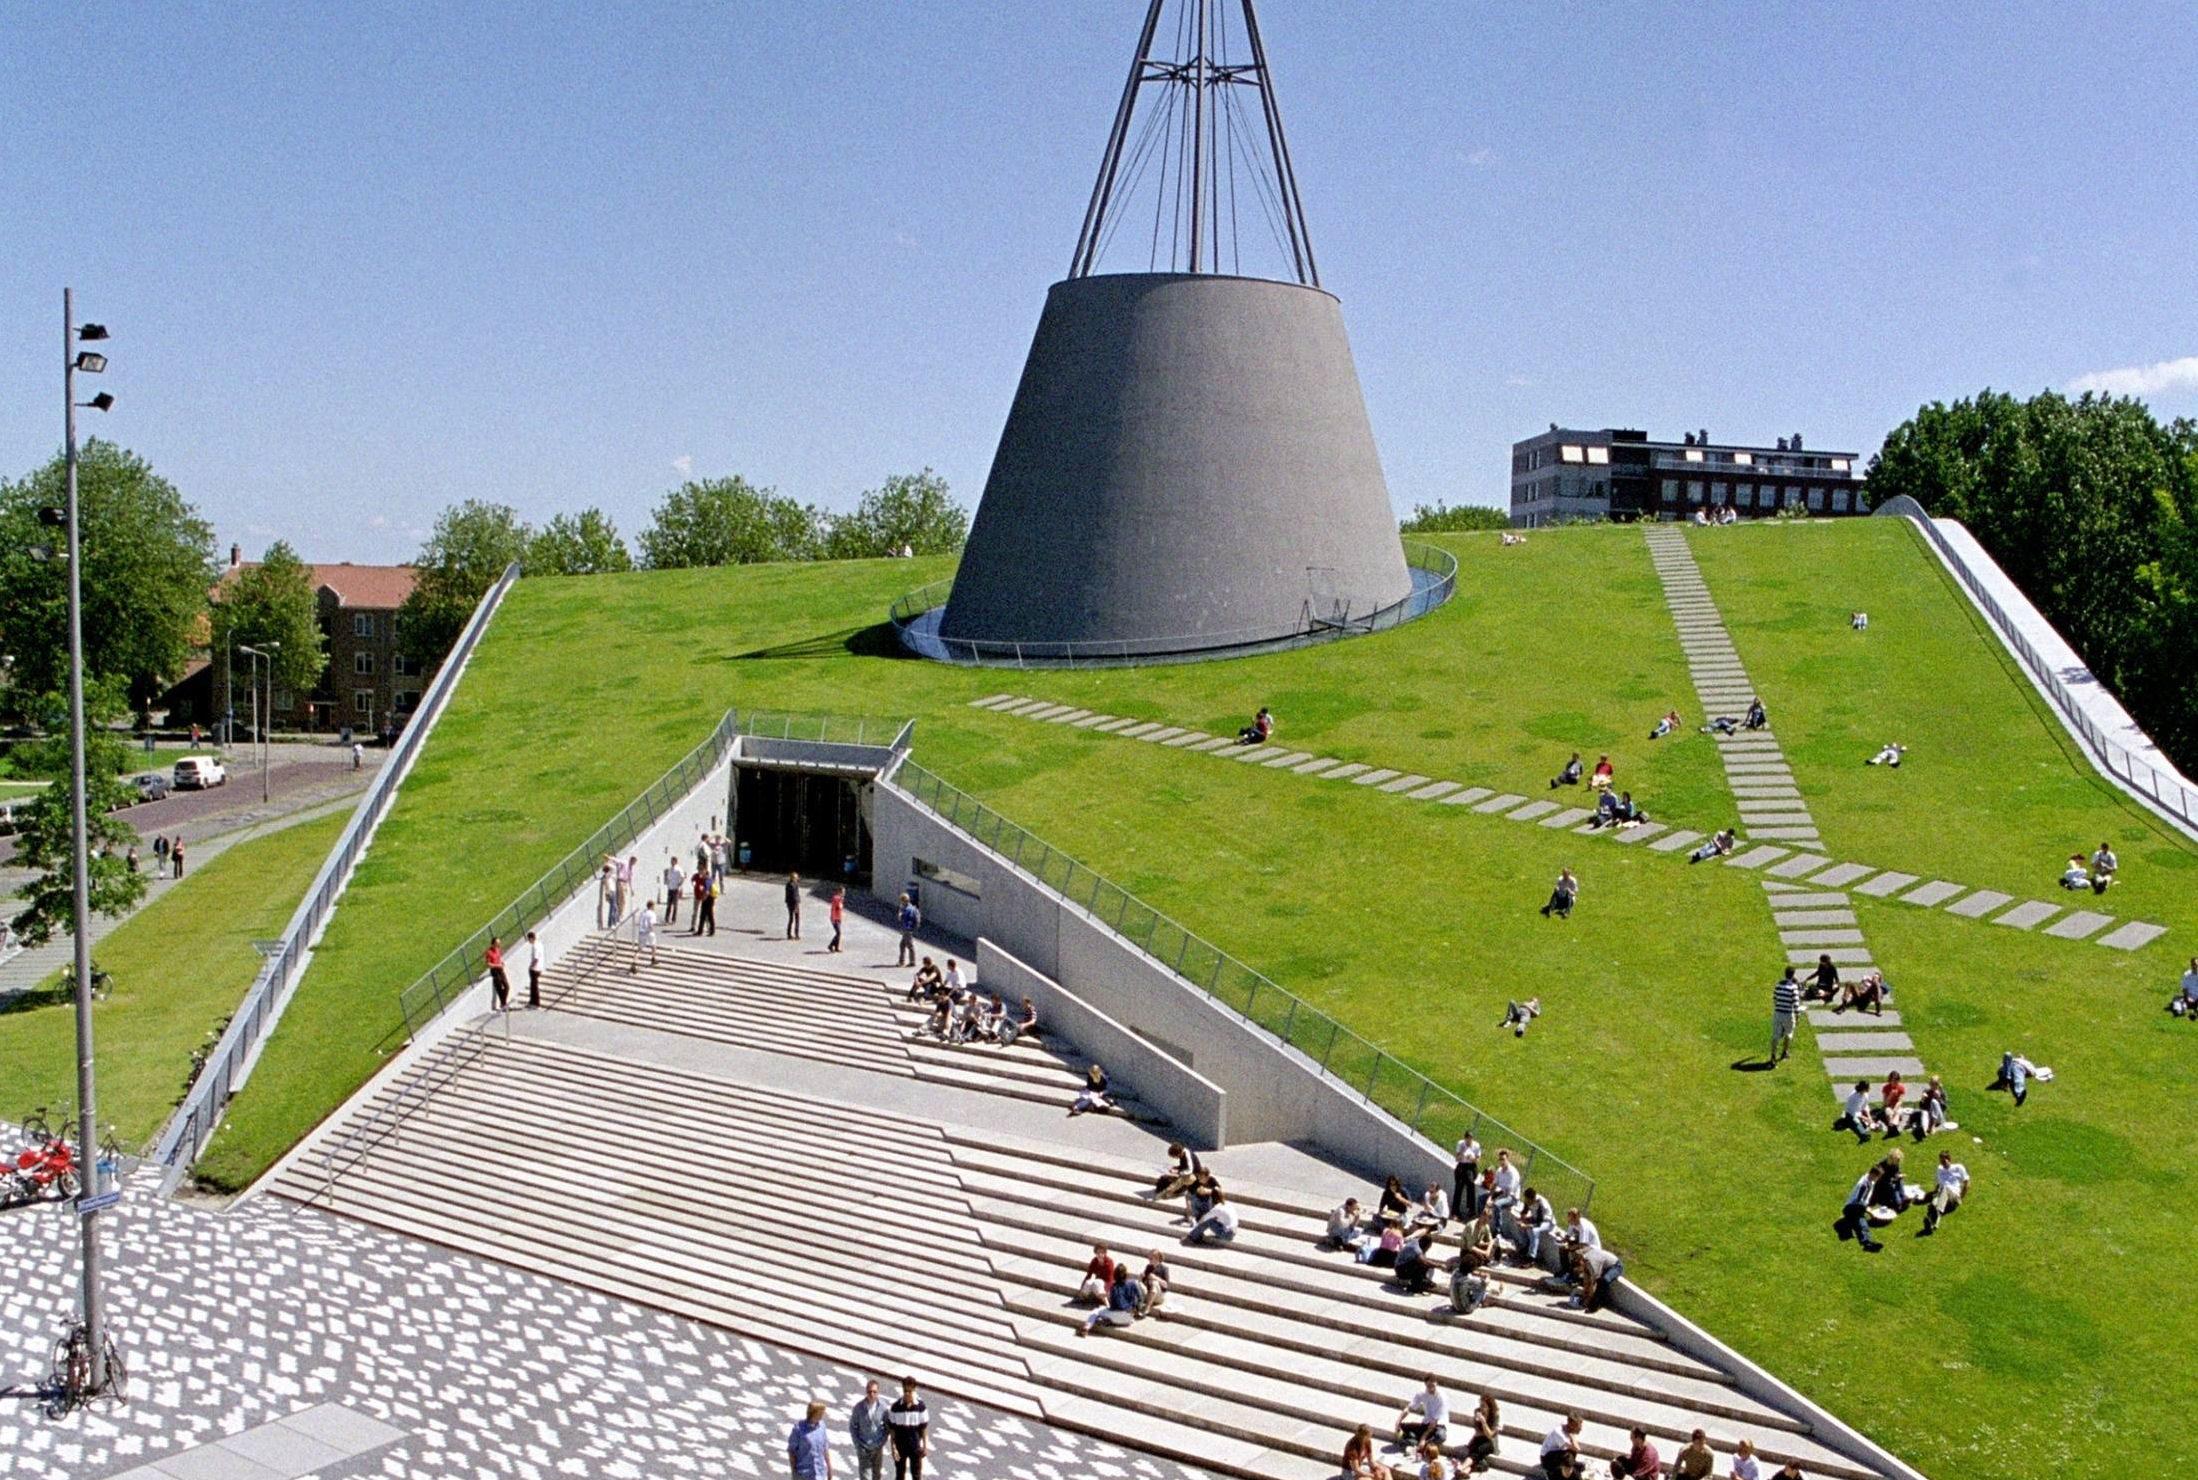
\includegraphics[height=8.65cm]{TUDelft/background-titlepage.jpg}};

            % hide the navigation things.
            \fill [cyan!95!black!70!blue] (0,2.9) -- (0,5.35) -- (-.5,5.35) -- (-.5,2.9) -- cycle ;%squareNorthWest
            \draw [fill=black] (0,0) -- (11,0) -- (11,2.9) -- (0,2.9) -- cycle ;
            %\fill [fill=cyan!65!blue!80] (7,-3.9) -- (12.4,-3.9) -- (12.4,-3.65) -- (7,-3.65) -- cycle;

            \node [shift={(0.8cm,-3.1cm)},textlabel,right,text width=10cm]  at (current page.north west) {\textbf{\large{\textrm{\titel}}}};
            \node [shift={(0.8cm,-4cm)},textlabel,cyan!95!black!70!blue,right,text width=10cm]  at (current page.north west)
            {\textbf{\large{\scriptsize \textrm{\subkop}}}};
            \node [shift={(0.8cm,-4.6cm)},textlabel,right]  at (current page.north west)
            {\normalsize{\naam}};
            \node [shift={(0.8cm,-5cm)},textlabel,right]  at (current page.north west)
            {\normalsize{\today}};
        \end{tikzpicture}};
    \end{tikzpicture}
\end{frame}
%==============================================================

\begin{frame}
  \frametitle{Content of presentation}

\end{frame}

\begin{frame}
  \frametitle{Planners}

  What is a Planner?

  \begin{itemize}
    \item From \alert{initial state}
    \item To \alert{Goal state}
    \item Through \alert{Actions}
  \end{itemize}

\end{frame}

\begin{frame}
  \frametitle{Examples of a Planning Problem}

  \begin{tabular}{c c}
    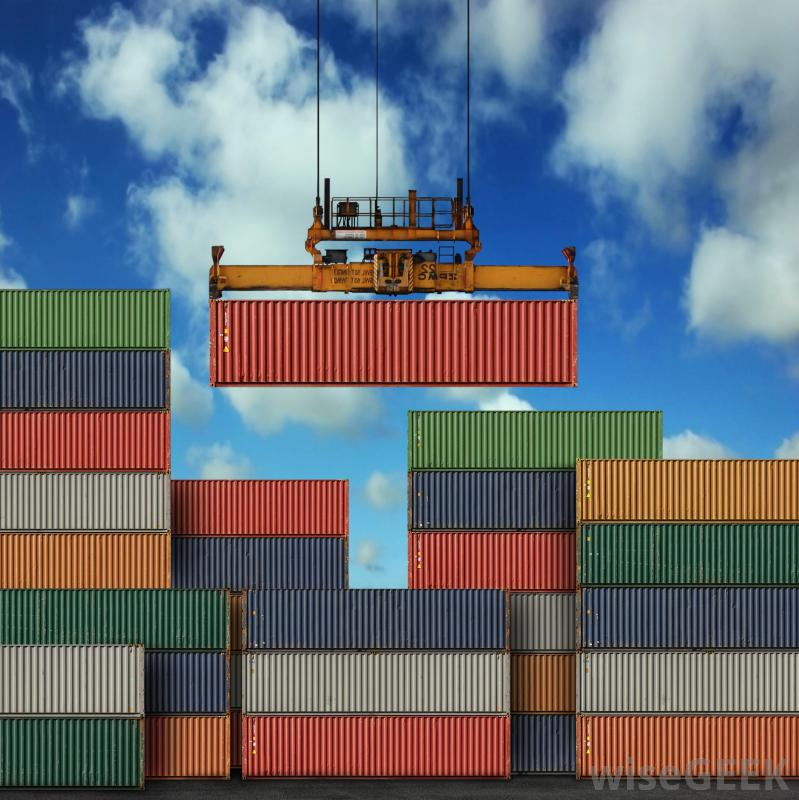
\includegraphics[width=3.5cm]{images/containers.jpg}     &
    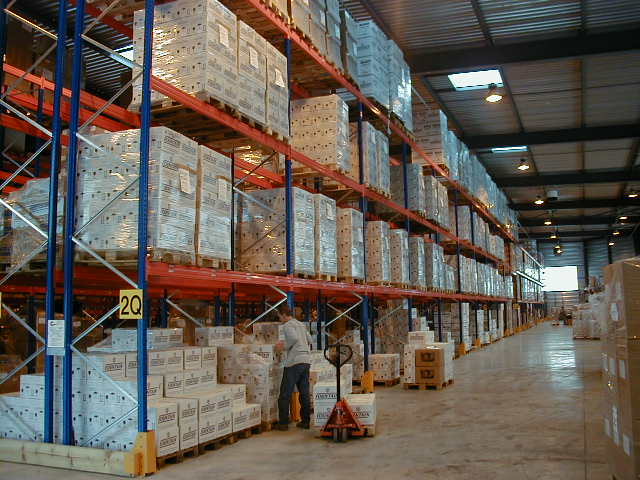
\includegraphics[width=3.5cm]{images/inventory.jpg}      \\
    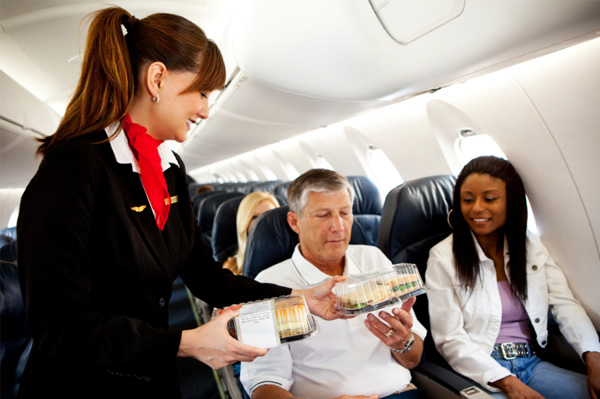
\includegraphics[width=3.5cm]{images/airplane-food.jpg}  &
    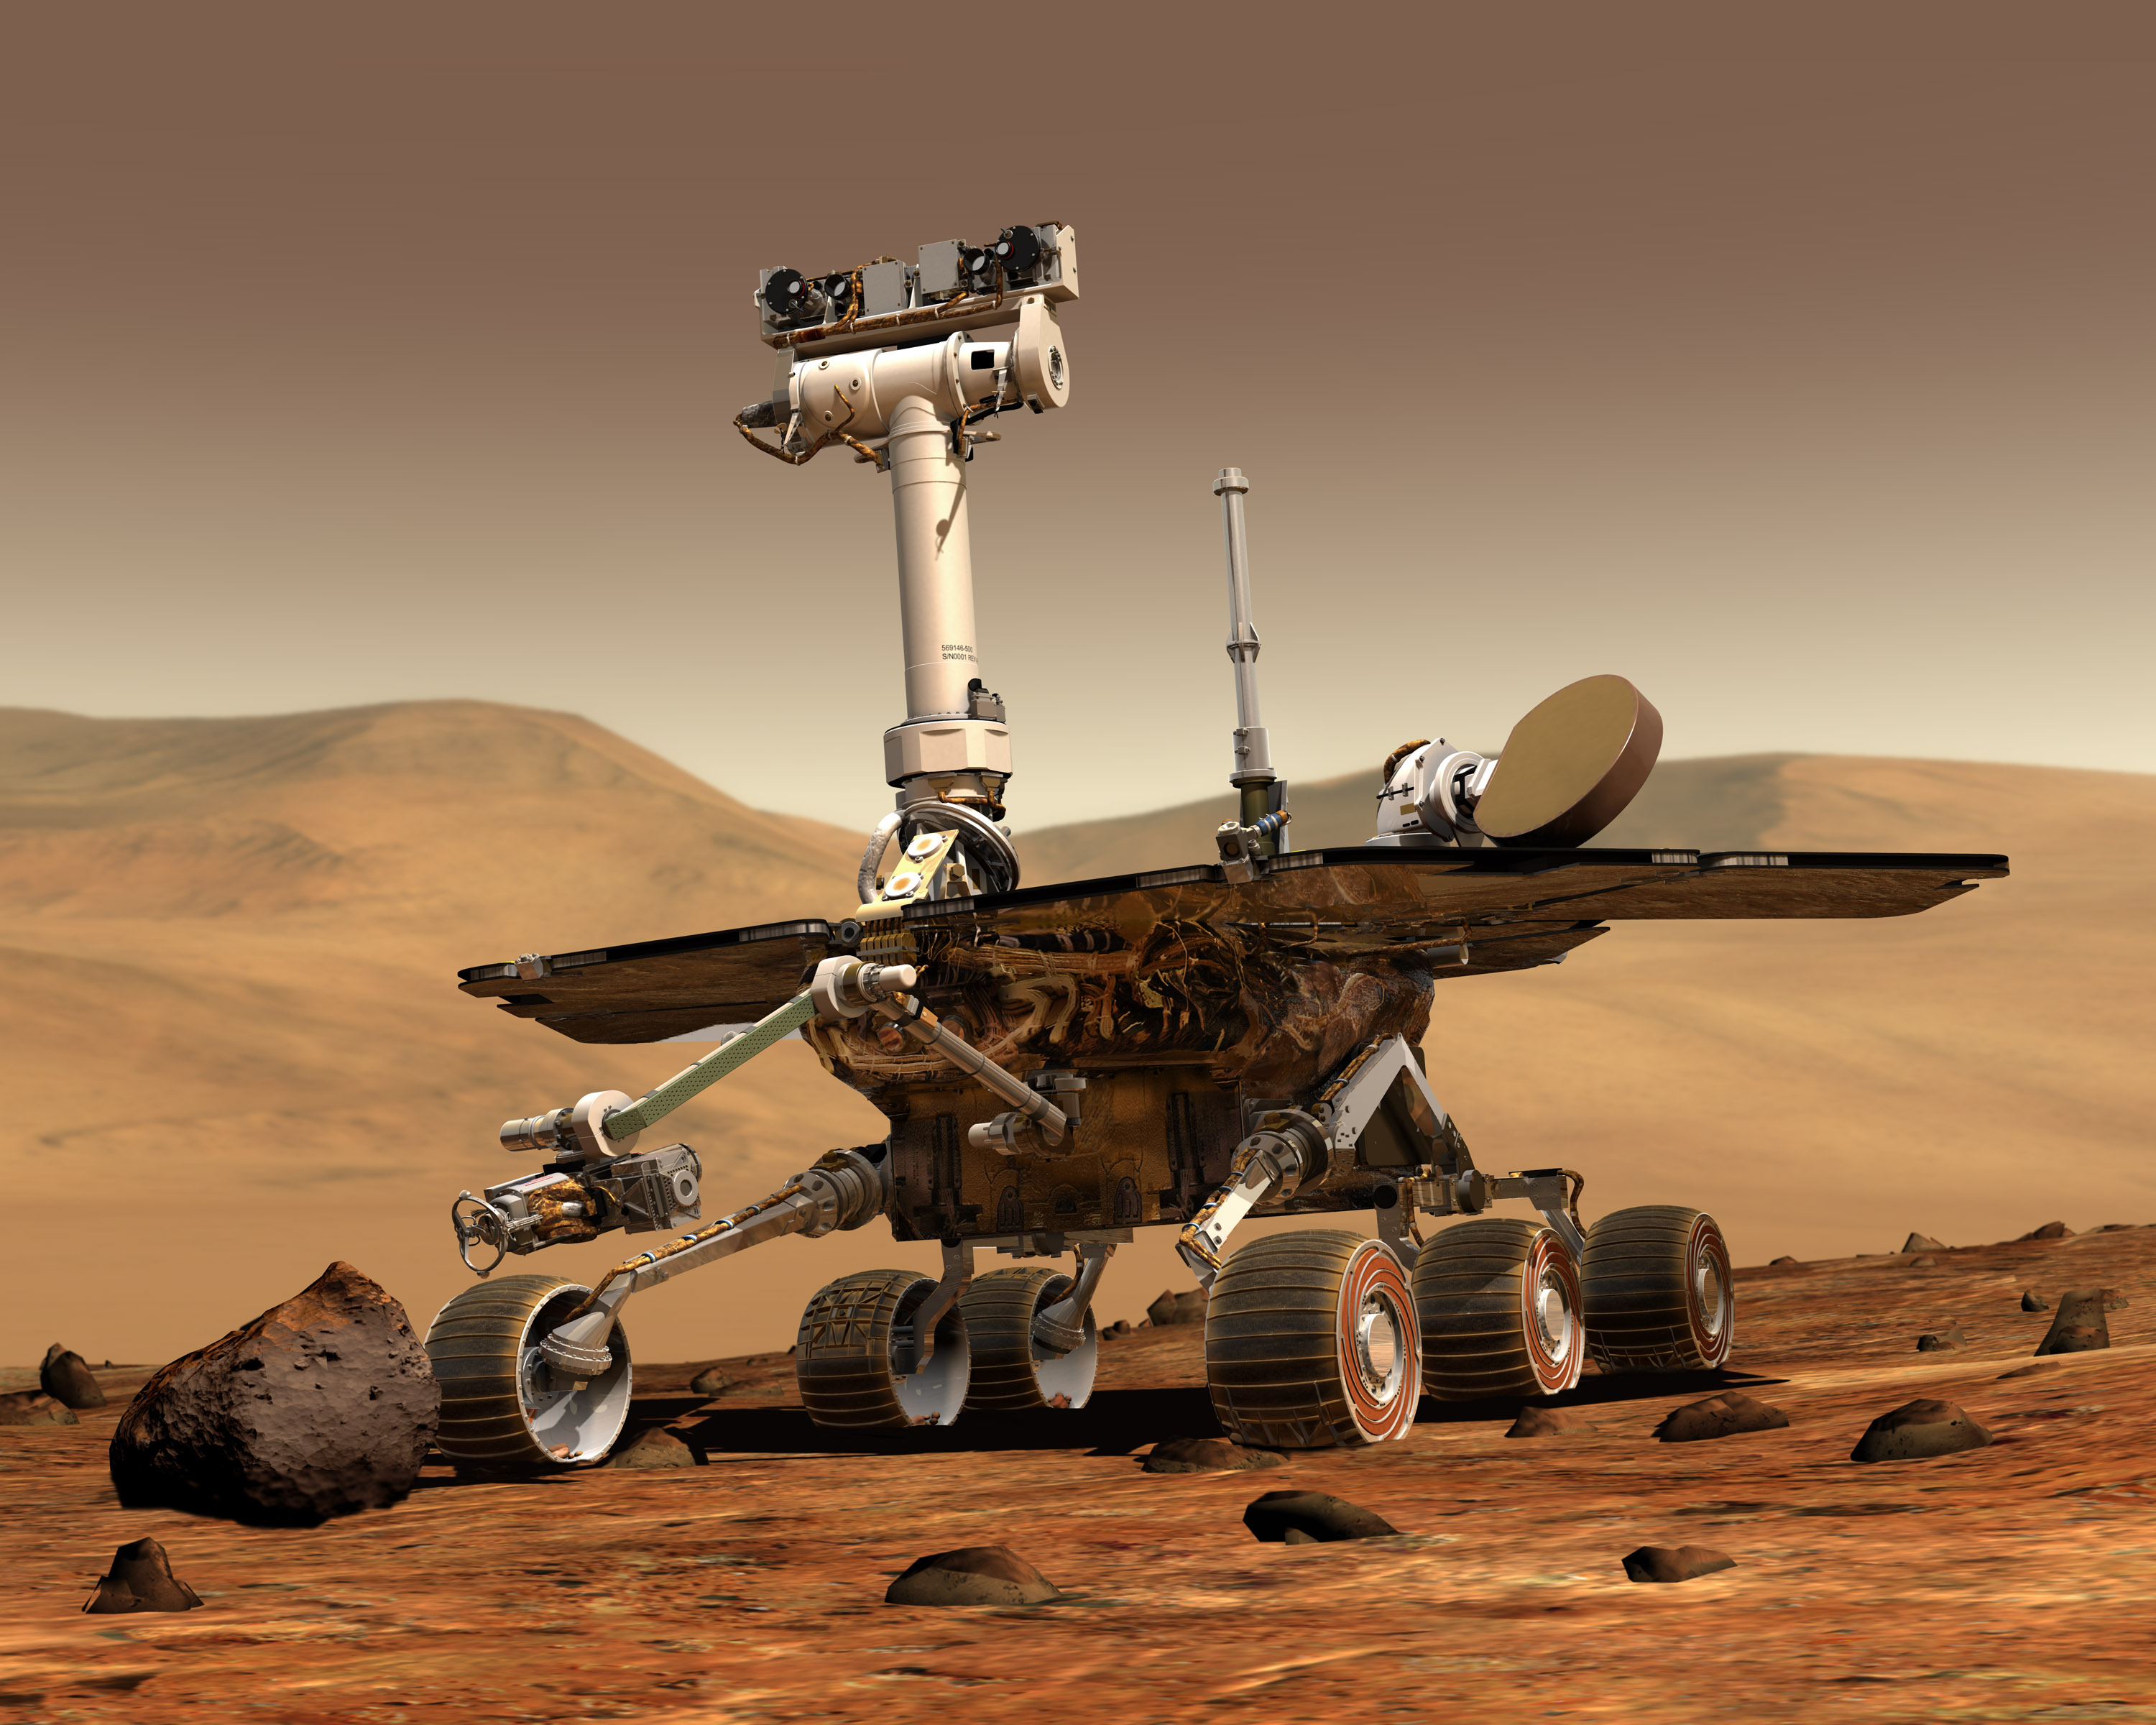
\includegraphics[width=3.5cm]{images/mars-rover.jpg}
  \end{tabular}

\end{frame}

\begin{frame}
  \frametitle{Classical Planning Example}

  \begin{columns}
    \column{0.3\textwidth}
    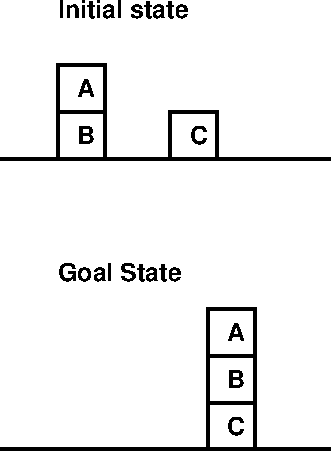
\includegraphics[width=\textwidth]{../presentation-plan/blocksworld.pdf}

    \column{0.7\textwidth}

    \begin{itemize}
      \item From initial state to goal state?
      \item Create a planning plan.
    \end{itemize}



  \end{columns}

\end{frame}

\begin{frame}
  \frametitle{Planning with Uncertainty}
\end{frame}

\begin{frame}
  \frametitle{Historical background information}
\end{frame}

\begin{frame}
  \frametitle{Planning under uncertainty: FF-Replan}
\end{frame}

\begin{frame}
  \frametitle{Planning under uncertainty: RFF}
\end{frame}

\begin{frame}
  \frametitle{Planning under uncertainty: FF-Replan vs. RFF}
\end{frame}



\againframe{titlepage}

\end{document}
